\documentclass{standalone}
\usepackage{tikz}
\usetikzlibrary{patterns, positioning}
\usetikzlibrary{shapes.misc}
\usepackage[outline]{contour}
\contourlength{1.5pt} 


\begin{document}
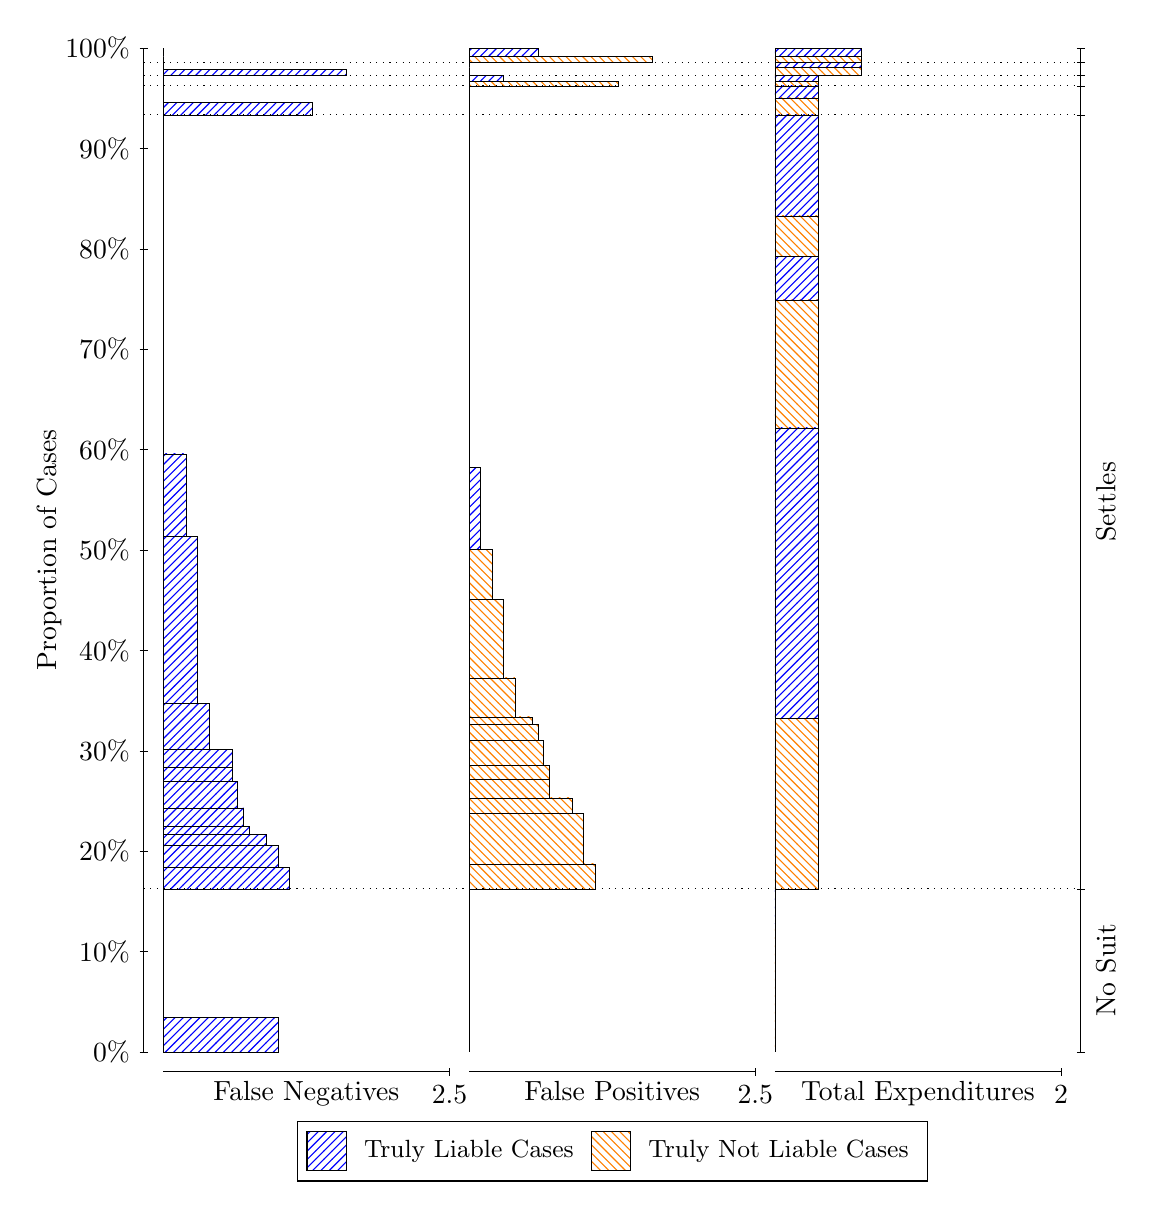
\begin{tikzpicture}
\draw[black, very thin] (1.5,1.75) -- (1.5,14.5);
\node[rotate=90, text=black, anchor=center] at (0.3, 8.125) {Proportion of Cases};
\draw[black, very thin] (1.45,1.75) -- (1.55,1.75);
\node[text=black, anchor=east] at (1.45, 1.75) {0\%};
\draw[black, very thin] (1.45,3.025) -- (1.55,3.025);
\node[text=black, anchor=east] at (1.45, 3.025) {10\%};
\draw[black, very thin] (1.45,4.3) -- (1.55,4.3);
\node[text=black, anchor=east] at (1.45, 4.3) {20\%};
\draw[black, very thin] (1.45,5.575) -- (1.55,5.575);
\node[text=black, anchor=east] at (1.45, 5.575) {30\%};
\draw[black, very thin] (1.45,6.85) -- (1.55,6.85);
\node[text=black, anchor=east] at (1.45, 6.85) {40\%};
\draw[black, very thin] (1.45,8.125) -- (1.55,8.125);
\node[text=black, anchor=east] at (1.45, 8.125) {50\%};
\draw[black, very thin] (1.45,9.4) -- (1.55,9.4);
\node[text=black, anchor=east] at (1.45, 9.4) {60\%};
\draw[black, very thin] (1.45,10.675) -- (1.55,10.675);
\node[text=black, anchor=east] at (1.45, 10.675) {70\%};
\draw[black, very thin] (1.45,11.95) -- (1.55,11.95);
\node[text=black, anchor=east] at (1.45, 11.95) {80\%};
\draw[black, very thin] (1.45,13.225) -- (1.55,13.225);
\node[text=black, anchor=east] at (1.45, 13.225) {90\%};
\draw[black, very thin] (1.45,14.5) -- (1.55,14.5);
\node[text=black, anchor=east] at (1.45, 14.5) {100\%};

\draw[black, very thin] (13.4,1.75) -- (13.4,14.5);
\draw[black, very thin] (13.35,1.75) -- (13.45,1.75);
\node[anchor=west] at (13.35, 1.75) {};
\draw[black, very thin] (13.35,3.8214) -- (13.45,3.8214);
\node[anchor=west] at (13.35, 3.8214) {};
\draw[black, very thin] (13.35,13.652) -- (13.45,13.652);
\node[anchor=west] at (13.35, 13.652) {};
\draw[black, very thin] (13.35,14.02) -- (13.45,14.02);
\node[anchor=west] at (13.35, 14.02) {};
\draw[black, very thin] (13.35,14.156) -- (13.45,14.156);
\node[anchor=west] at (13.35, 14.156) {};
\draw[black, very thin] (13.35,14.32) -- (13.45,14.32);
\node[anchor=west] at (13.35, 14.32) {};
\draw[black, very thin] (13.35,14.5) -- (13.45,14.5);
\node[anchor=west] at (13.35, 14.5) {};

\draw[black, very thin, pattern color=blue, pattern=north east lines] (1.75,1.75) rectangle (3.2033,2.1942);
\draw[black, very thin, pattern color=orange, pattern=north west lines] (1.75,2.1942) rectangle (1.75,3.8214);
\draw[black, very thin, pattern color=blue, pattern=north east lines] (1.75,3.8214) rectangle (3.3487,4.0904);
\draw[black, very thin, pattern color=blue, pattern=north east lines] (1.75,4.0904) rectangle (3.2033,4.3748);
\draw[black, very thin, pattern color=blue, pattern=north east lines] (1.75,4.3748) rectangle (3.058,4.5174);
\draw[black, very thin, pattern color=blue, pattern=north east lines] (1.75,4.5174) rectangle (2.84,4.6192);
\draw[black, very thin, pattern color=blue, pattern=north east lines] (1.75,4.6192) rectangle (2.7673,4.8513);
\draw[black, very thin, pattern color=blue, pattern=north east lines] (1.75,4.8513) rectangle (2.6947,5.1837);
\draw[black, very thin, pattern color=blue, pattern=north east lines] (1.75,5.1837) rectangle (2.622,5.3603);
\draw[black, very thin, pattern color=blue, pattern=north east lines] (1.75,5.3603) rectangle (2.622,5.5936);
\draw[black, very thin, pattern color=blue, pattern=north east lines] (1.75,5.5936) rectangle (2.3313,6.1773);
\draw[black, very thin, pattern color=blue, pattern=north east lines] (1.75,6.1773) rectangle (2.186,8.2943);
\draw[black, very thin, pattern color=blue, pattern=north east lines] (1.75,8.2943) rectangle (2.0407,9.345);
\draw[black, very thin, pattern color=orange, pattern=north west lines] (1.75,9.345) rectangle (1.75,13.652);
\draw[black, very thin, pattern color=blue, pattern=north east lines] (1.75,13.652) rectangle (3.6393,13.805);
\draw[black, very thin, pattern color=orange, pattern=north west lines] (1.75,13.805) rectangle (1.75,14.02);
\draw[black, very thin, pattern color=orange, pattern=north west lines] (1.75,14.02) rectangle (1.75,14.08);
\draw[black, very thin, pattern color=blue, pattern=north east lines] (1.75,14.08) rectangle (1.75,14.156);
\draw[black, very thin, pattern color=blue, pattern=north east lines] (1.75,14.156) rectangle (4.0753,14.224);
\draw[black, very thin, pattern color=orange, pattern=north west lines] (1.75,14.224) rectangle (1.75,14.32);
\draw[black, very thin, pattern color=orange, pattern=north west lines] (1.75,14.32) rectangle (1.75,14.391);
\draw[black, very thin, pattern color=blue, pattern=north east lines] (1.75,14.391) rectangle (1.75,14.5);
\draw[black, very thin, pattern color=orange, pattern=north west lines] (5.6333,1.75) rectangle (5.6333,3.3772);
\draw[black, very thin, pattern color=blue, pattern=north east lines] (5.6333,3.3772) rectangle (5.6333,3.8214);
\draw[black, very thin, pattern color=orange, pattern=north west lines] (5.6333,3.8214) rectangle (7.232,4.138);
\draw[black, very thin, pattern color=orange, pattern=north west lines] (5.6333,4.138) rectangle (7.0867,4.7828);
\draw[black, very thin, pattern color=orange, pattern=north west lines] (5.6333,4.7828) rectangle (6.9413,4.9775);
\draw[black, very thin, pattern color=orange, pattern=north west lines] (5.6333,4.9775) rectangle (6.6507,5.2108);
\draw[black, very thin, pattern color=orange, pattern=north west lines] (5.6333,5.2108) rectangle (6.6507,5.3914);
\draw[black, very thin, pattern color=orange, pattern=north west lines] (5.6333,5.3914) rectangle (6.578,5.7101);
\draw[black, very thin, pattern color=orange, pattern=north west lines] (5.6333,5.7101) rectangle (6.5053,5.9079);
\draw[black, very thin, pattern color=orange, pattern=north west lines] (5.6333,5.9079) rectangle (6.4327,6.0043);
\draw[black, very thin, pattern color=orange, pattern=north west lines] (5.6333,6.0043) rectangle (6.2147,6.5017);
\draw[black, very thin, pattern color=orange, pattern=north west lines] (5.6333,6.5017) rectangle (6.0693,7.4968);
\draw[black, very thin, pattern color=orange, pattern=north west lines] (5.6333,7.4968) rectangle (5.924,8.1283);
\draw[black, very thin, pattern color=blue, pattern=north east lines] (5.6333,8.1283) rectangle (5.7787,9.1791);
\draw[black, very thin, pattern color=blue, pattern=north east lines] (5.6333,9.1791) rectangle (5.6333,13.652);
\draw[black, very thin, pattern color=orange, pattern=north west lines] (5.6333,13.652) rectangle (5.6333,13.866);
\draw[black, very thin, pattern color=blue, pattern=north east lines] (5.6333,13.866) rectangle (5.6333,14.02);
\draw[black, very thin, pattern color=orange, pattern=north west lines] (5.6333,14.02) rectangle (7.5227,14.08);
\draw[black, very thin, pattern color=blue, pattern=north east lines] (5.6333,14.08) rectangle (6.0693,14.156);
\draw[black, very thin, pattern color=orange, pattern=north west lines] (5.6333,14.156) rectangle (5.6333,14.252);
\draw[black, very thin, pattern color=blue, pattern=north east lines] (5.6333,14.252) rectangle (5.6333,14.32);
\draw[black, very thin, pattern color=orange, pattern=north west lines] (5.6333,14.32) rectangle (7.9587,14.391);
\draw[black, very thin, pattern color=blue, pattern=north east lines] (5.6333,14.391) rectangle (6.5053,14.5);
\draw[black, very thin, pattern color=orange, pattern=north west lines] (9.5167,1.75) rectangle (9.5167,3.3772);
\draw[black, very thin, pattern color=blue, pattern=north east lines] (9.5167,3.3772) rectangle (9.5167,3.8214);
\draw[black, very thin, pattern color=orange, pattern=north west lines] (9.5167,3.8214) rectangle (10.062,5.9874);
\draw[black, very thin, pattern color=blue, pattern=north east lines] (9.5167,5.9874) rectangle (10.062,9.6748);
\draw[black, very thin, pattern color=orange, pattern=north west lines] (9.5167,9.6748) rectangle (10.062,11.301);
\draw[black, very thin, pattern color=blue, pattern=north east lines] (9.5167,11.301) rectangle (10.062,11.855);
\draw[black, very thin, pattern color=orange, pattern=north west lines] (9.5167,11.855) rectangle (10.062,12.369);
\draw[black, very thin, pattern color=blue, pattern=north east lines] (9.5167,12.369) rectangle (10.062,13.652);
\draw[black, very thin, pattern color=orange, pattern=north west lines] (9.5167,13.652) rectangle (10.062,13.866);
\draw[black, very thin, pattern color=blue, pattern=north east lines] (9.5167,13.866) rectangle (10.062,14.02);
\draw[black, very thin, pattern color=orange, pattern=north west lines] (9.5167,14.02) rectangle (10.062,14.08);
\draw[black, very thin, pattern color=blue, pattern=north east lines] (9.5167,14.08) rectangle (10.062,14.156);
\draw[black, very thin, pattern color=orange, pattern=north west lines] (9.5167,14.156) rectangle (10.607,14.252);
\draw[black, very thin, pattern color=blue, pattern=north east lines] (9.5167,14.252) rectangle (10.607,14.32);
\draw[black, very thin, pattern color=orange, pattern=north west lines] (9.5167,14.32) rectangle (10.607,14.391);
\draw[black, very thin, pattern color=blue, pattern=north east lines] (9.5167,14.391) rectangle (10.607,14.5);
\draw[black, dotted] (1.5,3.8214) -- (13.4,3.8214);
\draw[black, dotted] (1.5,13.652) -- (13.4,13.652);
\draw[black, dotted] (1.5,14.02) -- (13.4,14.02);
\draw[black, dotted] (1.5,14.156) -- (13.4,14.156);
\draw[black, dotted] (1.5,14.32) -- (13.4,14.32);
\draw[black, very thin] (1.75,1.5) -- (5.3833,1.5);
\node[text=black, anchor=north] at (3.5667, 1.5) {False Negatives};
\draw[black, very thin] (5.3833,1.45) -- (5.3833,1.55);
\node[text=black, anchor=north] at (5.3833, 1.45) {2.5};

\draw[black, very thin] (5.6333,1.5) -- (9.2667,1.5);
\node[text=black, anchor=north] at (7.45, 1.5) {False Positives};
\draw[black, very thin] (9.2667,1.45) -- (9.2667,1.55);
\node[text=black, anchor=north] at (9.2667, 1.45) {2.5};

\draw[black, very thin] (9.5167,1.5) -- (13.15,1.5);
\node[text=black, anchor=north] at (11.333, 1.5) {Total Expenditures};
\draw[black, very thin] (13.15,1.45) -- (13.15,1.55);
\node[text=black, anchor=north] at (13.15, 1.45) {2};

\node[text=black, centered, rotate=90] at (13.72, 2.7857) {\contour{white}{No Suit}};
\node[text=black, centered, rotate=90] at (13.72, 8.7367) {\contour{white}{Settles}};





\draw (7.449999999999999,1.5) node[draw=none] (baseCoordinate) {};
\begin{scope}[align=center]
        \matrix[scale=0.5, draw=black, below=0.5cm of baseCoordinate, nodes={draw}, column sep=0.1cm]{
            \node[rectangle, draw, minimum width=0.5cm, minimum height=0.5cm, pattern color=blue, pattern=north east lines] {}; &
            \node[draw=none, font=\small, text=black] (B) {Truly Liable Cases}; &
            \node[rectangle, draw, minimum width=0.5cm, minimum height=0.5cm, pattern color=orange, pattern=north west lines] {}; &
            \node[draw=none, font=\small, text=black] (B) {Truly Not Liable Cases}; \\
            };
\end{scope}

\end{tikzpicture}
\end{document}